% Chapter Template
% cSpell:words parencite 
\chapter{Marco teórico} % Main chapter title 

\label{Chapter2} % Change X to a consecutive number; for referencing this chapter elsewhere, use \ref{ChapterX}
En este capítulo se comprenderán conceptos teóricos sobre las tecnologías claves en las cuales se basa el proyecto. Como introducción, se analizará el funcionamiento de las redes tradicionales, donde se dejará en evidencia la necesidad de un nuevo paradigma. 

Luego, se analizarán los fundamentos en los que se basan las Redes Definidas por Software y por qué este paradigma resuelve los problemas presentados por el enfoque de las redes tradicionales. 

También, se introducirán conceptos de lenguajes de modelado y se abordará la importancia de la gestión de la red. Se estudiará \textit{NETCONF} como protocolo de gestión de red. Finalmente, se abordan conceptos de dispositivos ópticos de transporte.

%----------------------------------------------------------------------------------------
%	SECTION 1
%----------------------------------------------------------------------------------------
\section{Redes tradicionales} \label{sec:rdtr}

La infraestructura actual de las redes tradicionales basan su funcionamiento íntegramente en los dispositivos de red \parencite{ISACA}. Cada dispositivo lleva su propia gestión sobre el plano de datos y el plano de control de manera local y comunica a los demás dicha información de ser necesario. 

Un ejemplo de esto se puede observar en la figura \ref{fig:dev_tradicional}, donde dos dispositivos intercambian información referente al plano de control.


\begin{figure}[H]
	\centering
	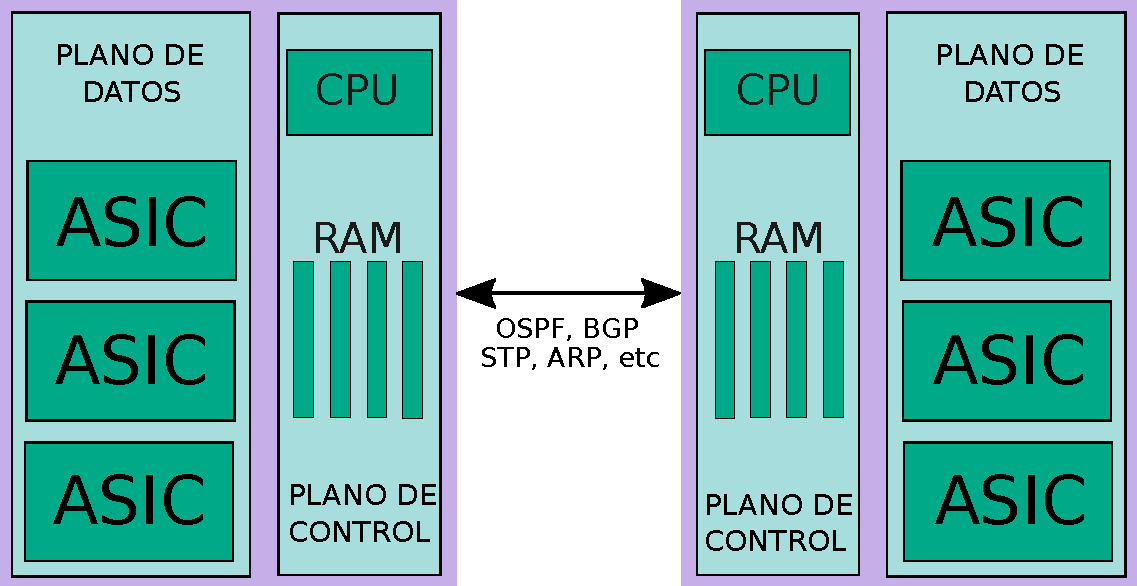
\includegraphics[scale=0.60]{Figures/dispositivo-tradicional.pdf}
	\caption{Comportamiento de dispositivos en redes tradicionales.}
	\label{fig:dev_tradicional}
  \end{figure}


\subsection{Plano de Control}
Comprende la configuración del sistema, la administración y el intercambio de información de ruteo entre los dispositivos \parencite{ControlPlane}. Es el responsable de administrar la configuración del equipo y de programar el camino que será usado para el flujo de los paquetes. En otras palabras, es en este plano donde se calculan y se toman las decisiones de enrutamiento y reenvío. En las redes tradicionales, cualquier aplicación que utilice el dispositivo para administrar su configuración reside en esta capa. 

El proceso de establecimiento de la topología de red utilizando un plano de control que se ejecuta localmente, es compleja debido a que no existe ningún dispositivo que sea conocido por toda la red. Para gestionar cambios o actualizaciones en cada dispositivo se debe estar conectado a su plano de control de forma individual, lo que no resulta en un enfoque inteligente.

\subsection{Plano de Datos}
También conocido como plano de usuario o plano de reenvío \parencite{DataPlane}, es el encargado de transportar el tráfico de usuario hacia el destinatario final. Tiene como objetivo el reenvío de los paquetes hacia el próximo salto basándose en las decisiones tomadas por la capa de control.
\\


El enfoque dado por las redes tradicionales cumplió con las necesidades de una época donde las arquitecturas cliente-servidor eran dominantes. Tiene como ventaja ser simple a nivel lógico, mientras que el plano de control implica el uso de microprocesadores para tratar los paquetes y conformar las tablas, el plano de datos se desarrolla en silicio. A pesar de ello, presenta una serie de problemas \parencite{onfwhitepaper}:

\begin{itemize}
	\item \textbf{Funcionalidad de la red integrada en los dispositivos:} El plano de control se encuentra íntegramente en los dispositivos de red, lo que resulta en una configuración de red estática, inflexible y descentralizada. 
	\item \textbf{Escalabilidad:} La escalabilidad resulta afectada y no apropiada para la explosión de las nuevas tecnologías como \textit{Big Data}, \textit{Cloud Computing} y el \textit{Streaming}, donde la complejidad de la red incrementa rápidamente debido a que cada dispositivo agregado debe ser configurado y administrado.
	\item \textbf{Políticas inconsistentes:} Si las políticas de configuración cambian a nivel de red, implica un cambio en todos los dispositivos que la componen por parte de los administradores de red.
	\item \textbf{Dependencia del fabricante y personalización:} El plano de control integrado a los dispositivos de red resulta en una dependencia a los ciclos de producción de equipamientos por parte de los fabricantes para incorporar nuevas funcionalidades. Además, con la finalidad de asegurar la calidad de servicio y brindar alta perfomance, la industria define los protocolos de red de forma específica y aislada, sin el beneficio de una acción conjunta e incapacitando a los operadores a personalizar la red para sus entornos individuales y específicos. 
\end{itemize}

%----------------------------------------------------------------------------------------
%	SECTION 2
%----------------------------------------------------------------------------------------
\section{Redes Definidas por Software} \label{sec:rsdn}

A diferencia de las aplicaciones y los nuevos requerimientos de los usuarios, las redes no han cambiado mucho respecto a los últimos 30 años \parencite{sdnroad}. El desarrollo de las \textit{SDN} se inició en 1990 donde se introdujo el concepto de funciones programables en la red, teniendo gran innovación en 2001-2007 donde se propone separar el plano de datos del plano de control. El próximo gran paso de las \textit{SDN} llegó en 2007-2010, con la implementación de la \textit{API OpenFlow}.
\\

Las redes definidas por software nacen en respuesta a la dinámica y flexibilidad que requieren las nuevas tendencias, donde el enfoque presentado por las redes tradicionales no cumple dado su naturaleza estática. 

\subsection{Definición de \textit{SDN}}
Según la \textit{ONF} \parencite{onfwhitepaper}, la red definida por software, también conocida como red programable o automatizada, consiste en una arquitectura donde el plano de datos se encuentra separado del plano de control y donde este último a su vez puede controlar varios dispositivos.

Tal como destaca \textit{SDx Central} en su reporte \parencite{SDXCentralReport}, este nuevo paradigma presenta las siguientes ventajas:

\begin{itemize}
	\item \textbf{Plano de control centralizado:} A diferencia del enfoque presentado por las redes tradicionales donde se tenía un plano de control distribuido entre los diferentes equipos que conforman la red, ahora se tiene un plano de control centralizado y presente a nivel lógico en un mismo punto. De esta forma, se tiene una visión general y global de toda la red, relajando las comunicaciones entre los dispositivos y las complejidades introducidas por las configuraciones individuales de cada uno. Además, el plano de control ahora es directamente programable, sin tener que usar como intermediario el plano de datos. Todo el tráfico ahora está bajo la supervisión de este nuevo plano de control centralizado, transformando a la red en una red programable. 
	\item \textbf{Costos:} Los costos relacionados al control de la gestión del tráfico y de configuración de los diferentes equipos se ven reducidos en tiempo y esfuerzo dado el plano de control centralizado.
	\item \textbf{Automatización:} Un beneficio indirecto de tener un plano de control centralizado, es poder tomar diferentes decisiones y políticas en base a la visibilidad global de la red en tiempo real, aplicando configuraciones en los diferentes equipos de forma automática.
	\item \textbf{Escalabilidad:} \textit{SDN} admite topologías dinámicas con capacidades para adaptarse a cambios, debido a la automatización de la configuración de los dispositivos. Con la capacidad de ajustar los picos y las bajas en la carga del tráfico, las empresas pueden crear e implementar nuevos servicios y aplicaciones sin demora debido a la infraestructura más flexible.
	\item \textbf{Mantenimiento y monitoreo:} Por medio del controlador \textit{SDN} se puede conocer, en cualquier momento, el estado actual de la red incluyendo los dispositivos que la componen.
	\item \textbf{Seguridad:} Dado que la administración de toda la red se realiza en un solo punto, se asegura que no existan debilidades o inconsistencias en las configuraciones de las aplicaciones y los equipos.
\end{itemize}

\subsection{Arquitectura de \textit{SDN}}
En las redes tradicionales, cada dispositivo tiene integrado tanto el plano de datos como el plano de control. En \textit{SDN}, el plano de datos se encuentra desacoplado del plano de control y, además, se puede diferenciar un nuevo plano llamado \textit{plano de aplicación} \parencite{onfsdnarq}. A continuación, se analizará cuál es la función que cumple cada plano en esta nueva arquitectura propuesta por las \textit{SDN}.

\subsubsection{Plano de Datos}
Comprende la misma funcionalidad que en las redes tradicionales. Consiste en un conjunto de dispositivos de red con funcionalidades de reenvío de paquetes.

\subsubsection{Plano de Aplicación}
Con el enfoque de las redes tradicionales, el plano de aplicación se encontraba integrado en el plano de control. En \textit{SDN}, el plano de aplicación se desacopla al igual que el plano de control. En este plano se encuentran las aplicaciones de red que implementan las funcionalidades de más alto nivel y que participan en las decisiones de administración y control de ruteo.

\subsubsection{Plano de Control}
Toda la función de control se encuentra centralizada fuera de los dispositivos, permitiendo a los desarrolladores de aplicaciones utilizar las capacidades de la red pero haciendo una abstracción de su topología o sus funciones. Tiene como objetivo mediar, organizar y facilitar la comunicación entre los diferentes equipos y las aplicaciones. Además, este plano ahora está disponible para poder ser programado desde un software externo al controlador.
\\

En la figura \ref{fig:arquitectura_sdn}, se expone la anatomía de un controlador \textit{SDN}. En ella, se puede observar dos interfaces comprendidas por el plano de control \parencite{sdnarqsouth}: \textit{Southbound} y, \textit{Northbound}.

\begin{itemize}
	\item \textbf{\textit{Southbound API}:} necesaria por la separación del plano de control del plano de datos. Define la \textit{API} de comunicación entre el controlador y los diferentes dispositivos de red, en otras palabras, entre el plano de control y el plano de datos.  
	\item \textbf{\textit{Northbound API}:} funciona como interfaz tanto de alto como de bajo nivel, es necesaria para permitir que las aplicaciones que se ejecutan en la parte superior de \textit{SDN} puedan comunicarse con el mismo. En el primer caso, la interfaz provee una abstracción de la red en sí misma, permitiendo a los desarrolladores no tener que preocuparse por los dispositivos individuales, sino manejar la red como un todo. En el segundo caso, la interfaz advierte a las aplicaciones sobre la existencia de los dispositivos individuales y sus enlaces, pero oculta las diferencias entre los dispositivos. 
\end{itemize}


\begin{figure}[htbp]
	\centering
	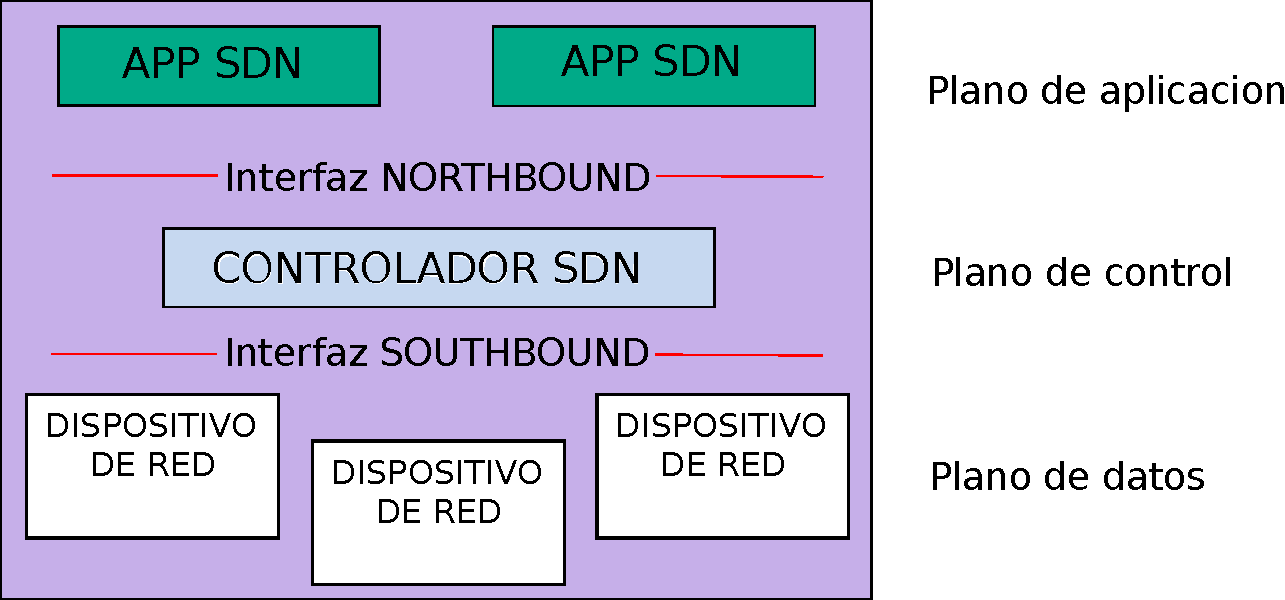
\includegraphics[scale=0.6]{Figures/arquitectura-controlador.pdf}
	\caption{Arquitectura de un controlador \textit{SDN} tradicional.}
	\label{fig:arquitectura_sdn}
  \end{figure}

%----------------------------------------------------------------------------------------
%	SECTION 3
%----------------------------------------------------------------------------------------
\section{Gestión de la Red} \label{sec:gestionred}
En la actualidad se puede encontrar una gran variedad de redes, desde pequeñas redes domésticas de intranet hasta redes empresariales o de proveedores de servicios. Cada una de estas redes tienen diversos requerimientos de gestión.  Las pequeñas redes domésticas, que consisten en unos pocos dispositivos conectados, requieren una sobrecarga de administración baja, y con frecuencia, pueden gestionarse manualmente de forma eficiente. No así las redes más grandes, que podrían contener cientos dispositivos conectados requiriendo un enfoque más sistemático para hacer frente a las complejidades que surgen debido al tamaño de la red. A medida que la red crece en estructura y complejidad, se hace evidente la necesidad de una solución eficiente para la gestión de la misma \parencite{gestionderedes}.

\subsection{Protocolos de Gestión}
Existen múltiples formas de llevar a cabo la administración de la configuración en los diversos dispositivos que conforman la red. En esta sección, se analizarán dos alternativas: \textit{CLI} y \textit{SNMP}.

\subsubsection{\textit{Command Line Interface}}

\textit{CLI} es el enfoque más común en el ámbito de gestión de la configuración, adoptado por múltiples empresas. Consiste en un método para comunicarse con las aplicaciones que la subyacen, a través de una interfaz de usuario simple basada en texto. De esta forma, permite que el administrador pueda ingresar instrucciones en una línea de comandos a través de una terminal y recibir las respuestas en la misma. La aplicación subyacente es la encargada de procesar la instrucción y devolver alguna respuesta al usuario. Generalmente, las respuestas están orientadas a que resulten fácil de entender para las personas, sin embargo, no se encuentran orientadas a las API’s, ya que no existe un formato o un estándar de cómo representar dichas respuestas. Además, las implementaciones internas podrían ser diferentes entre los distintos dispositivos, incluso entre dispositivos del mismo fabricante, de modo que, tanto los comandos como las respuestas podrían variar significativamente entre los equipos.
\\

Un ejemplo de una operación en \textit{CLI} puede verse en la figura \ref{lstlisting:cli}. La primer línea ingresada, hace referencia a un acceso al modo de configuración de un dispositivo cualquiera. En la segunda, se agrega una entrada estática a la tabla de ruteo y en la tercera se abandona el modo de configuración.

\begin{lstlisting}[language=SHELXL, caption=Interacción tipica con un dispositivo mediante \textit{CLI}., label=lstlisting:cli]
	> configure terminal
	#> ip route 192.0.2.0/8 ethernet 1/2 192.0.2.4
	#> !
\end{lstlisting}


  Este enfoque presenta una serie desventajas \parencite{clilimitacion}. En primer lugar, la implementación de las aplicaciones subyacentes a la \textit{CLI} no están estandarizadas, por lo que las operaciones varían drásticamente entre dispositivos de diferentes fabricantes e incluso en implementaciones \textit{CLI} del mismo fabricante. A su vez, los fabricantes podrían brindar una actualización de software del dispositivo, donde los comandos \textit{CLI} de la versión anterior se vean modificados o eliminados, lo que no solo se traduce a problemas para el administrador de red, sino también para las \textit{API’s} que hagan uso de la \textit{CLI}. 
  \\

  En segundo lugar, realizar un cambio en el estado de un dispositivo podría requerir múltiples transacciones, y en el caso de que alguna de estas falle, el dispositivo podría quedar en un estado inconsistente. Por ejemplo, en la figura \ref{lstlisting:cli} se observó que para realizar una operación sencilla como agregar una entrada a la tabla de ruteo, implicó el uso de al menos tres comandos. De forma similar, podrían existir operaciones que requieran de transacciones con una mayor cantidad de instrucciones. \textit{CLI} no define de forma estándar una solución para deshacer los cambios aplicados en el dispositivo.

  \subsubsection{\textit{Simple Network Management Protocol}}
  \textit{SNMP} es un protocolo de monitoreo y administración de red, estandarizado por primera vez en 1988 por la \textit{IETF} \parencite{snmprfc}. Su funcionamiento se basa en una arquitectura cliente-servidor, donde los mensajes se intercambian a través del protocolo de transporte no orientado a la conexión \textit{UDP}. Consiste en una colección de agentes y administradores formando entre ellos una red, donde se denomina administrador a aquel dispositivo que tiene el rol de ejecutar aplicaciones de administración de red, mientras que los dispositivos que requieran ser administrados se denominan agentes \parencite{snmprfcfunc}.

  Las capacidades para administrar la red en \textit{SNMP} quedan representadas en lo que se conoce como \textit{MIB}. Una \textit{MIB} es una base de datos que contiene información jerárquica y estructurada en forma de árbol de todos los parámetros gestionables de la red. 
  Dicha base de datos se debe cargar en el administrador \textit{SNMP}, para ello cada agente \textit{SNMP} expone al administrador \textit{SNMP} una serie de módulos \textit{MIB}. Con esta información el administrador podría alterar dinámicamente la configuración del agente. 
  \\

  El uso de \textit{SNMP} como monitoreo es una práctica común desde su publicación, sin embargo, se desalentó su uso en áreas de gestión de configuración por las siguientes razones \parencite{snmplimitacion}: 

  \begin{itemize}
	\item Problemas inherentes al protocolo de transporte \textit{UDP}, donde los mensajes pueden perderse o llegar desordenados, así como también la falta de mecanismos de seguridad para los mismos jugaron un papel importante para reemplazar \textit{SNMP} por otros protocolos de administración de red.
	\item No existe una estandarización de los módulos \textit{MIB} para configurar las funciones de red. El trabajo de descubrir correctamente los módulos \textit{MIB} para cada dispositivo es tarea del usuario, lo que resulta compleja y no eficiente.
\end{itemize}

La figura \ref{fig:snmpfig} muestra las operaciones más comunes de \textit{SNMP}.

\begin{figure}[htbp]
	\centering
	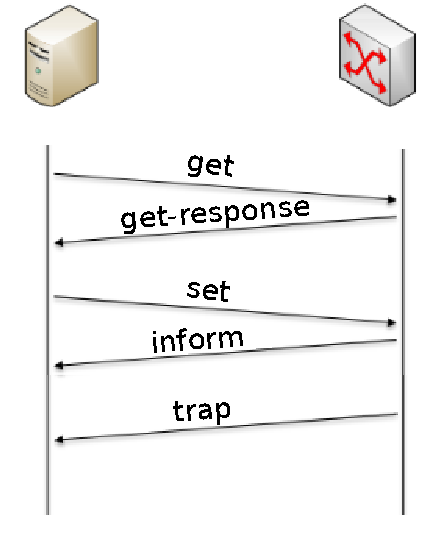
\includegraphics[scale=0.8]{Figures/snmp_ejemplo.pdf}
	\caption{Operaciones tipicas en \textit{SNMP}.}
	\label{fig:snmpfig}
  \end{figure}

\subsubsection{Otras alternativas}
Algunos enfoques para la gestión de la red pueden incluir soluciones basadas en páginas web, que permiten al administrador modificar las configuraciones en el dispositivo de forma gráfica y más amigable, pero generalmente resultan más limitadas que las \textit{CLI}. 
Además, algunos dispositivos pueden brindar soluciones propietarias para la gestión de la configuración, sin embargo, estas soluciones suelen ser muy específicas a un dispositivo o una familia de dispositivos, y rara vez suelen ser compatibles entre sí. Estos últimos también representan una carga para los administradores, donde cada solución requiere que el administrador aprenda otra manera de configurar las funcionalidades de la red.  

\subsection{\textit{NETCONF}}
Esta sección repasa brevemente los conceptos y características principales que ofrece el protocolo \textit{NETCONF}. Además, aspectos de seguridad, transporte y control de acceso del protocolo se discuten en detalle. 

\subsubsection{Definición}
\textit{NETCONF} fue estandarizado por la \textit{IETF} por primera vez en el 2006, en el \textit{RFC 4741} \parencite{netconfrfc}. Actualmente está siendo adoptado por los principales proveedores de dispositivos de red y ha ganado el apoyo de la industria. Según detalla Carl Moberg \parencite{netconfusos}, podemos encontrar que fabricantes como Juniper, Huawei, Cisco, entre otros, brindan soporte desde hace tiempo del protocolo \textit{NETCONF}. 
\\

La \textit{IETF} definde a \textit{NETCONF} como un protocolo estándar para Instalar, manipular y borrar configuraciones en un dispositivo \parencite{netconfrfcnuevo}. Permite implementar una \textit{API} formal utilizando el lenguaje de modelado \textit{YANG} para administrar y monitorear las funcionalidades de la red. \textit{NETCONF} utiliza el paradigma de las \textit{RPC}, donde construye los mensajes que intercambian información como un flujo con codificación \textit{XML}. Funciona con una arquitectura cliente-servidor, donde los mensajes son transportados utilizando algún protocolo orientado a la conexión. El \textit{RFC 6241}, en la sección 1.2, menciona una partición conceptual del protocolo en cuatro capas, dicha partición se refleja en la figura \ref{fig:netconf}. 
\\

A continuación, se explica qué función cumple cada una de estas capas.

\begin{itemize}
	\item \textbf{Capa de transporte seguro:} provee mecanismos de comunicación entre cliente y servidor.  
	\item \textbf{Capa de mensajes:} encargada de la codificación y partición de los mensajes.  
	\item \textbf{Capa de operación:} define las operaciones admitidas por el protocolo.
	\item \textbf{Capa de contenido:} relaciona la representación y el modelado de los datos en el protocolo.    
\end{itemize}

\begin{figure}[htbp]
	\centering
	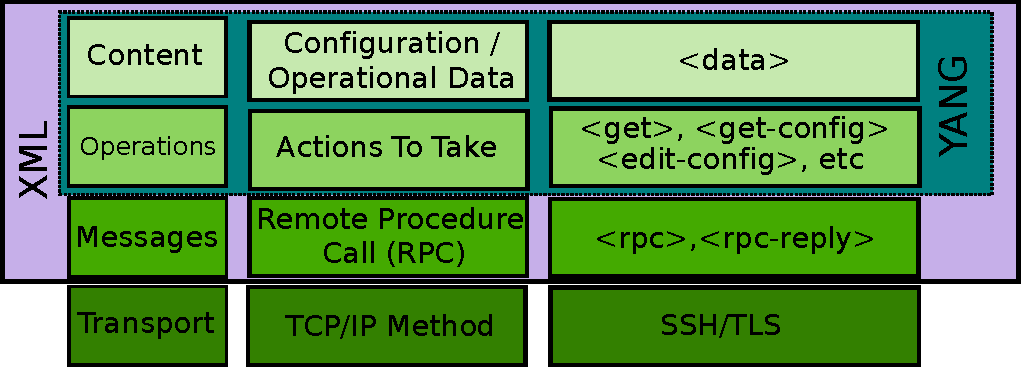
\includegraphics[scale=0.8]{Figures/stack-netconf.pdf}
	\caption{Separación conceptual del protocolo \textit{NETCONF}.}
	\label{fig:netconf}
  \end{figure}


  Las características que destacan a \textit{NETCONF} como protocolo de administración de red son \parencite{netconfpros}:

  \begin{itemize}
	\item Capacidad de restauración de los datos y \textit{backup} de la configuración.
	\item De uso fácil, presentando la información de forma estructurada con una codificación entendible para las personas y las \textit{API’s}.
	\item Implementa mecanismos de control de errores mediante validación de sintaxis y semántica.
	\item Separación clara de los datos de configuración y los datos de estado.
	\item Posibilidad de gestionar la configuración en un dispositivo de manera reactiva mediante notificaciones del mismo.
\end{itemize}

\textit{NETCONF} separa los datos de configuración de los datos de estado de un dispositivo. Según lo detallado en la sección 1.1. y 1.4 del \textit{RFC 6242}, se define a cada uno como:

\begin{itemize}
	\item \textbf{Datos de configuración:} información que se puede leer o escribir y que se utiliza para llevar al dispositivo de un estado inicial a un estado deseado. Un ejemplo es la velocidad del ventilador del cpu del dispositivo.  
	\item \textbf{Datos de estado:} representa información de sólo lectura y estadísticas brindadas por el dispositivo. Por ejemplo, la temperatura del cpu del equipo.   
\end{itemize}

\subsubsection{Conceptos del Protocolo}
Como se mencionó anteriormente, \textit{NETCONF} define un protocolo de administración de red con arquitectura cliente-servidor, donde el cliente en este caso es el sistema de administración de la red o el administrador del sistema, mientras que el dispositivo que contiene una o más funciones de red que deben ser administradas, actúa de servidor. El cliente y el servidor inician la sesión de protocolos mediante un primer mensaje que da lugar al intercambio de capacidades o \textit{capabilities}, donde se definen qué operaciones estarán disponibles para su uso. Este primer mensaje recibe el nombre de \textit{HELLO} \parencite{netconfrfcnuevo}. La figura \ref{fig:netconf_comunicacion} ejemplifica la arquitectura presentada por el protocolo.

\begin{figure}[htbp]
	\centering
	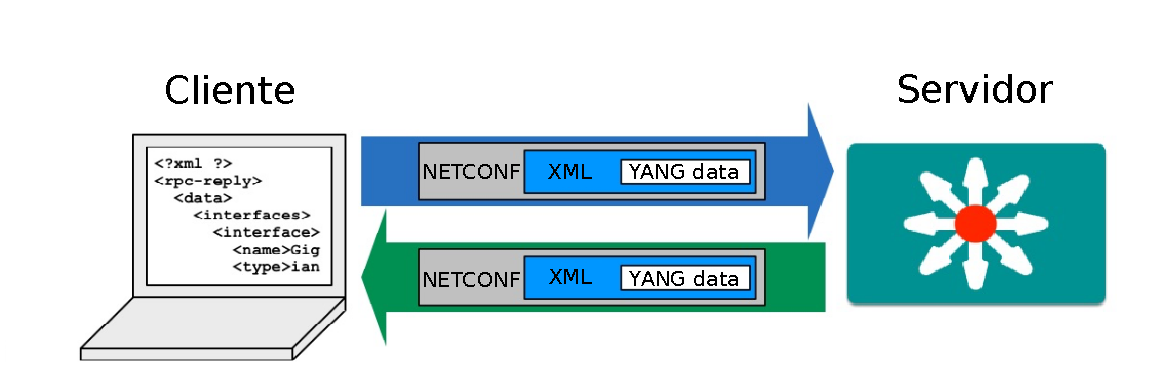
\includegraphics[scale=0.8]{Figures/netconf-cliente-servidor.pdf}
	\caption{Arquitectura cliente-servidor en el protocolo \textit{NETCONF}.}
	\label{fig:netconf_comunicacion}
  \end{figure}

  \subsubsection{Capacidades}
  El protocolo \textit{NETCONF} está diseñado para ser altamente extensible y, con este fin, es compatible con el intercambio inicial de capacidades entre cliente y servidor \parencite{netconfrfcnuevo}. Este intercambio de información permite al cliente ajustar sus comportamientos basándose en las funcionalidades que admite el servidor. Cada capacidad establecida por el protocolo recibe un nombre asignado por la \textit{IANA}. Además, también se incluye el intercambio de los modelos \textit{YANG} que tiene implementado el servidor, lo cual es necesario no solo para que el cliente pueda aprender de los mismos, sino también para reconocer las diferentes revisiones implementadas en el servidor. 
  \\
  
  La utilidad de esta característica reside en que, a través del intercambio de las capacidades entre el cliente y el servidor, el protocolo define cuáles serán las operaciones admitidas desde el inicio de la sesión, evitando así el ingreso de comandos de configuración incorrectos o no soportados. 


  \subsubsection{Sesión orientada a la conexión}
  La sección dos del \textit{RFC 6242}, referida a protocolos de transporte, detalla que \textit{NETCONF} no esta vinculado a ningún protocolo de transporte específico. El requisito necesario de \textit{NETCONF} para el protocolo de transporte subyacente es que el mismo sea orientado a la conexión. 
  \\

  Esta es una de las principales ventajas frente a \textit{SNMP}, donde los mensajes en este último eran transportados a través del protocolo no orientado a la conexión, \textit{UDP}. Además, el hecho de que \textit{NETCONF} no especifique el uso de un único protocolo de transporte orientado a la conexión, se traduce a una mayor flexibilidad y personalización para el administrador, pudiendo optar por aquella que mejor se ajuste a las necesidades de los equipos involucrados.


  \subsubsection{Sesión orientada a la autenticación}
  El protocolo \textit{NETCONF} es orientado a la sesión con autenticación, utilizando una arquitectura cliente-servidor donde el servidor escucha un puerto asignado para recibir las conexiones con los clientes. 

  Según la sección dos del \textit{RFC 6242} referida a seguridad, el protocolo mínimamente debe ofrecer autenticación, confidencialidad e integridad. Cualquier mensaje \textit{NETCONF}, incluido el mensaje \textit{HELLO}, se envian unicamente si el cliente y servidor se han autenticado de forma correcta. No se especifica un protocolo en particular, pudiendo utilizarse alguno de los múltiples protocolos de transporte seguros existentes en la actualidad como \textit{TLS}, \textit{SSH}, \textit{BEEP}, etc. Cualquier implementación de \textit{NETCONF} debe, al menos, soportar \textit{SSH} como protocolo de transporte seguro.

  Además, según el \textit{RFC 6536} relacionado al control de acceso de usuarios, \textit{NETCONF} admite una jerarquía de niveles de usuarios. Por ejemplo, tener dos grupos de usuarios donde uno tenga permisos de configuración más limitados que el otro.

  \subsubsection{Bases de datos}
  \textit{NETCONF} define en la sección cinco del \textit{RFC 6242}, la existencia de uno o más \textit{datastores}, los cuales cumplen el papel de una base de datos conceptual que puede ser utilizada para almacenar y acceder tanto a los datos de configuración como a los datos de estado. El protocolo especifica y define tres tipos de base de datos: \textit{running}, \textit{startup} y \textit{candidate}, de las cuales únicamente es obligatorio que se implemente la primera. Si la implementación admite otras bases de datos, como por ejemplo \textit{startup} o \textit{candidate}, el servidor informará al cliente esta capacidad en el mensaje \textit{HELLO}. Cada operación en \textit{NETCONF} debe especificar la base de datos a la cual se realizará la consulta o modificación.
  \\

  A continuación, se detalla cada uno de los almacenes de datos mencionadas.
\begin{itemize}
	\item \textbf{\textit{startup}:} según lo especificado en la sección 8.7 del \textit{RFC 6242}, dicha base de datos se utiliza para almacenar de forma persistente la información de configuración del dispositivo. El contenido de esta es copiado de manera automática a la base de datos conocida como \textit{running} en el inicio del servidor \textit{NETCONF}. De esta forma, el protocolo brinda una herramienta al dispositivo para poder aplicar una configuración dado al inicio del equipo. 
	\item \textbf{\textit{running}:} refleja la configuración actualmente en uso por el dispositivo. Es la única base de datos conceptual que admite la presencia tanto de datos de estado como datos de configuración. A alto nivel, esta base de datos diferencia del estado de \textit{startup}, puesto que no es una configuración que será aplicada al inicio sino que refleja la configuración actual del dispositivo.
	\item \textbf{\textit{candidate}:} se encuentra definido en la sección 8.3 del \textit{RFC 6242}. Puede ser utilizado para realizar cambios que no se van a aplicar al dispositivo de forma directa, sino que lo harán una vez se realice un \textit{commit} sobre dicha base de datos. De esta forma, el contenido de \textit{candidate} es copiado a \textit{running}. Si de lo contrario se desea descartar los cambios realizados en este \textit{datastore}, la operación \textit{discard-changes} copia el contenido de \textit{running} a \textit{candidate}. En esta base de datos conceptual únicamente se admiten datos de configuración. En otras palabras, la utilidad de esta base de datos reside en que permite brindar al administrador un entorno de pruebas, donde se podría aplicar una configuración temporal en el equipo, con capacidad de volver a la configuración anterior en caso de fallas.
\end{itemize}


Como se mencionó anteriormente, cualquier implementación de \textit{NETCONF} debe admitir al menos el \textit{datastore running}, esto es necesario ya que los datos de estado (necesarios para monitorear el dispositivo) únicamente se encuentran admitidos en dicho \textit{datastore}.
\\

Por último, se podría hacer una analogía entre la separación de los datos de estado y los datos de configuración con la separación conceptual de dichas bases de datos lógicas. 
En el primer caso, se busca distinguir entre un dato de solo lectura de otro que admite la escritura, mientras que el segundo trata de diferenciar entre un conjunto de estados bien definidos que puede alcanzar el dispositivo. Por ejemplo, distinguir la configuración que va a aplicarse únicamente en el inicio del dispositivo a través del \textit{datastore startup}, de la configuración que podría llevar en un determinado momento a través del \textit{datastore running}.


\subsubsection{Operaciones del protocolo}

Las operaciones en el protocolo \textit{NETCONF} se definen como \textit{RPC} en los modelos \textit{YANG} relevantes. En dichos modelos también se definen los argumentos de entrada y los contenidos de salida para cada operación. Todas las operaciones están codificadas en \textit{XML} dentro de los mensajes \textit{RPC} que son, de hecho, los únicos mensajes que los clientes pueden enviar en las sesiones de \textit{NETCONF} después del intercambio inicial del mensaje \textit{HELLO}. 
\\

Como las operaciones son \textit{RPC}, cada mensaje enviado por los clientes tiene una respuesta por parte del servidor. Este resultado normalmente contiene \textit{ok} para indicar que la operación resultó según lo esperado, o \textit{error} indicando las razones por la cual falló dicha operación.
\\

El protocolo define en la sección 7 del \textit{RFC 6241} nueve operaciones básicas y necesarias para cualquier implementación del mismo, las cuales se describen a continuación:

\begin{itemize}
	\item \textbf{\textit{get}:} utilizado para consultar tanto datos de configuración como datos de estado al servidor \textit{NETCONF}.
	\item \textbf{\textit{get-config}:} operación que devuelve los datos de configuración del dispositivo. Puede incluir filtros para limitar la información enviada por parte del servidor.
	\item \textbf{\textit{edit-config}:} definida para crear, actualizar o borrar datos de configuración en el servidor. Únicamente se admite esta operación en las bases de datos \textit{running} o \textit{candidate}.
	\item \textbf{\textit{copy-config}:} crea o reemplaza completamente el contenido de una base de datos por otra. El caso de uso más común de esta operación es para copiar el contenido del \textit{datastore running} al \textit{datastore startup}. 
	\item \textbf{\textit{delete-config}:} Elimina completamente el contenido de un \textit{datastore} determinado. No se admite esta operación para la base de datos \textit{running}.
	\item \textbf{\textit{lock}:} permite al cliente bloquear la configuración completa de un \textit{datastore} específico en un dispositivo. Tales bloqueos son destinados a ser de corta duración, de esta forma un cliente puede realizar un cambio sin temor a la interacción con otros clientes de \textit{NETCONF}. Además, como el protocolo es orientado a la sesión, todos los recursos tomados por la misma tales como los datastores, deben ser liberados en el momento de la finalización o cierre de la sesión.
	\item \textbf{\textit{unlock}:} permite a la sesión liberar el recurso tomado por la operación lock.
	\item \textbf{\textit{close-session}:} utilizada para finalizar la sesión entre cliente y servidor \textit{NETCONF}. Cualquiera de las operaciones mencionadas en esta sección, quedan inhabilitadas una vez finalizada la sesión.
	\item \textbf{\textit{kill-session}:} permite al administrador de red finalizar alguna sesión inactiva que tiene recursos tomados. 
\end{itemize}

Además de estas nueve operaciones descritas por el protocolo, pueden proporcionarse operaciones adicionales basado en las capacidades anunciadas por el dispositivo, como por ejemplo operaciones \textit{RPC} definidas en los módulos \textit{YANG}.
\\

También, \textit{NETCONF} admite operaciones con capacidades más avanzadas. No es obligatorio que las diferentes implementaciones del mismo soporten las siguientes características, más bien, de hacerlo deben ser expuestas como capacidades admitidas en el mensaje \textit{HELLO}. Dichas operaciones se describen a continuación:
\begin{itemize}
	\item \textbf{\textit{commit}:} operación utilizada para copiar atómicamente el contenido del \textit{datastore candidate} al \textit{datastore running}. Además, puede incluirse la operación \textit{confirmed-commit}, esta última funciona como un \textit{backup} de la configuración previa al \textit{commit}, la cual se restablece al cabo de un \textit{timeout} si no se recibe la operación \textit{confirmed-commit}. \textit{NETCONF} describe a esta última como una “confirmación de la confirmación”.
	\item \textbf{\textit{discard-changes}:} revierte una operación que está en espera de confirmación. En otras palabras, se copia el contenido del \textit{datastore running} al \textit{datastore candidate}.
	\item \textbf{\textit{validate}:} consiste en una operación que verifica la correctitud semántica y sintáctica de una configuración antes de aplicar el cambio en el dispositivo. 
\end{itemize}


La tabla \ref{Tab:netconf_operaciones} resume las diferentes operaciones disponibles en \textit{NETCONF} y a qué \textit{datastore} podría aplicarse cada una de ellas. 
\\

\begin{table}[H]
	\centering
	\begin{tabular}{|c|c|c|}
	\hline
	\textbf{Capacicad}        & \textbf{Operación}                                                                                                       & \textbf{Base de datos afectada}                                                                                                                                     \\ \hline
	\textbf{writable-running} & \begin{tabular}[c]{@{}c@{}}lock\\ edit-config\\ unlock\\ copy-config\end{tabular}                                        & \begin{tabular}[c]{@{}c@{}}running\\ running\\ running\\ running -\textgreater startup\end{tabular}                                                                 \\ \hline
	\textbf{candidate}        & \begin{tabular}[c]{@{}c@{}}lock\\ edit-config\\ commit\\ validate\\ unlock\\ copy-config\end{tabular}                    & \begin{tabular}[c]{@{}c@{}}candidate\\ candidate\\ candidate -\textgreater running\\ candidate\\ candidate\\ running -\textgreater startup\end{tabular}             \\ \hline
	\textbf{confirmed-commit} & \begin{tabular}[c]{@{}c@{}}lock\\ edit-config\\ commit\\ confirmed-commit\\ validate\\ unlock\\ copy-config\end{tabular} & \begin{tabular}[c]{@{}c@{}}candidate\\ candidate\\ candidate\\ candidate -\textgreater running\\ candidate\\ candidate\\ running -\textgreater startup\end{tabular} \\ \hline
	\end{tabular}
	\caption{Ejemplo de operaciones disponibles en \textit{NETCONF}}
	\label{Tab:netconf_operaciones}
	\end{table}


  \subsubsection{Notificaciones}

  Si bien \textit{NETCONF} está diseñado principalmente para la administración de la configuración de la red mediante las operaciones expuestas anteriormente, existe una poderosa herramienta de monitoreo implementada en el protocolo llamada notificaciones. La \textit{RFC 5277} define a las mismas como un servicio de entrega de mensajes asíncronas a los clientes mediante suscripción. Esta característica no es obligatoria para las diferentes implementaciones del protocolo. De soportarlo, el servidor deberá comunicar a los clientes dicha característica como una capacidad del servidor en el mensaje \textit{HELLO}.
  \\

  Esta herramienta es similar a las notificaciones en el protocolo \textit{SNMP}, pero tiene la ventaja de que, en \textit{NETCONF}, el cliente puede especificar a qué notificación particular se desea suscribir, lo que permite un monitoreo más flexible. Además, como se mencionó anteriormente, el servidor puede declarar permisos para los diferentes usuarios y sesiones por lo que las notificaciones serán enviadas únicamente a aquellos clientes suscritos y que cumplan con el nivel de acceso requerido por el servidor.
  \\

  La importancia de las notificaciones reside en que los dispositivos de red tienen variables críticas que deben ser monitoreadas, por ejemplo la temperatura del equipo, el estado de los enlaces, la conectividad entre los mismos, etc. Dichas variables críticas reciben el nombre de alarmas. 
  
  De no existir un mecanismo de mensajes asíncronos, el monitoreo de las alarmas de un dispositivo podría implicar una sobrecarga en la red, debido a la cantidad de consultas periódicas que existirían sobre los dispositivos. 


  De esta forma, las notificaciones que define el protocolo \textit{NETCONF} no solo implica un monitoreo eficiente mediante mensajes asíncronos, sino que permite al protocolo poder tomar medidas de forma reactiva a las diferentes alarmas que se presenten. Por ejemplo, se podría configurar al cliente \textit{NETCONF} para que, de recibir una alarma de exceso de temperatura en el equipo, configure de forma automática una velocidad mayor en el ventilador del mismo. 
  \\

  Para finalizar, la figura \ref{fig:netconf_ejemplo} refleja una interacción típica entre cliente y servidor donde se observa el intercambio de capacidades en los mensajes \textit{HELLO}, el uso de diferentes operaciones con respuestas \textit{RPC} y las notificaciones.

  \begin{figure}[!h]
	\centering
	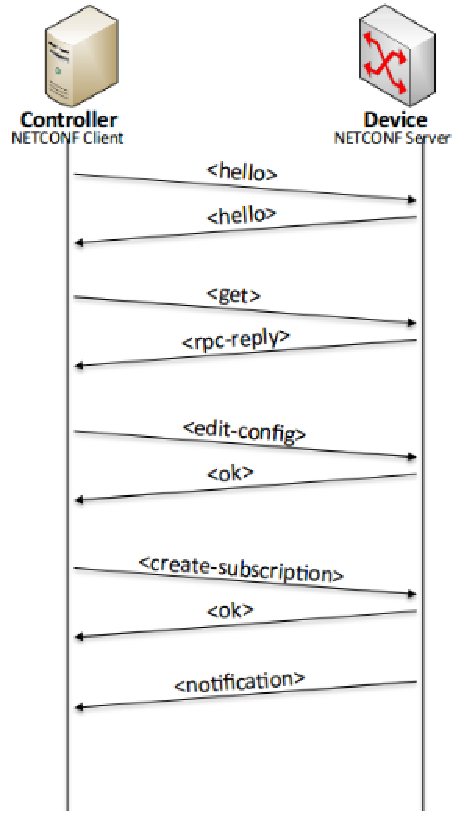
\includegraphics[scale=0.8]{Figures/netconf_ejemplo.pdf}
	\caption{Ejemplo de comunicación entre cliente y servidor NETCONF.}
	\label{fig:netconf_ejemplo}
  \end{figure}

  \subsection{Lenguaje de Modelado \textit{YANG}}
  Como se mencionó anteriormente, \textit{NETCONF} utiliza \textit{YANG} para modelar los datos de estado, los datos de configuración, las \textit{RPC} y las notificaciones. \textit{Yet Another Next Generation} es un lenguaje de modelado de datos desarrollado y estandarizado en la \textit{RFC 6020} por la \textit{IETF} en el año 2010 \parencite{yangrfc}. Si bien existen en la actualidad lenguajes de modelado como \textit{XML Schema}, \textit{SMI}, \textit{UML}, entre otros, la ventaja que presenta \textit{YANG} frente a los demás es que es un lenguaje de modelado específico para gestión de la configuración de red.

  \subsubsection{Conceptos del Lenguaje}
  \textit{YANG} define, en la sección 4.1 de la \textit{RFC 6020}, las funcionalidades de la red separando los datos de estado de los datos de configuración y presentando la información como una estructura de árbol jerárquica. Consiste en una serie de declaraciones y tipos que pueden ser usadas para definir los datos que se quieren modelar. Estas definiciones son contenidas en un módulo y describen qué tipo de datos admite una variable. A su vez, un módulo puede heredar definiciones de otro módulo.

  \subsubsection{Módulos y submódulos}
  Definen una estructura para el modelado de datos. Tienen un diseño predefinido que se debe seguir. Este diseño comienza con un encabezado, siguiendo de las declaraciones que contenga el módulo y por último las revisiones y comentarios respecto al mismo. 
  \\

  Se define el nombre del módulo, un prefijo para identificarlo, las dependencias, información de contacto al autor, descripción y revisiones. La declaración \textit{“include”} permite referenciar material que se describe en un submódulo, mientras que la declaración \textit{“import”} permite referenciar material que se encuentra descrito en un módulo externo. La estructura básica de un módulo puede verse en la figura \ref{fig:estructura_modulo}.

  \begin{figure}[htbp]
	\centering
	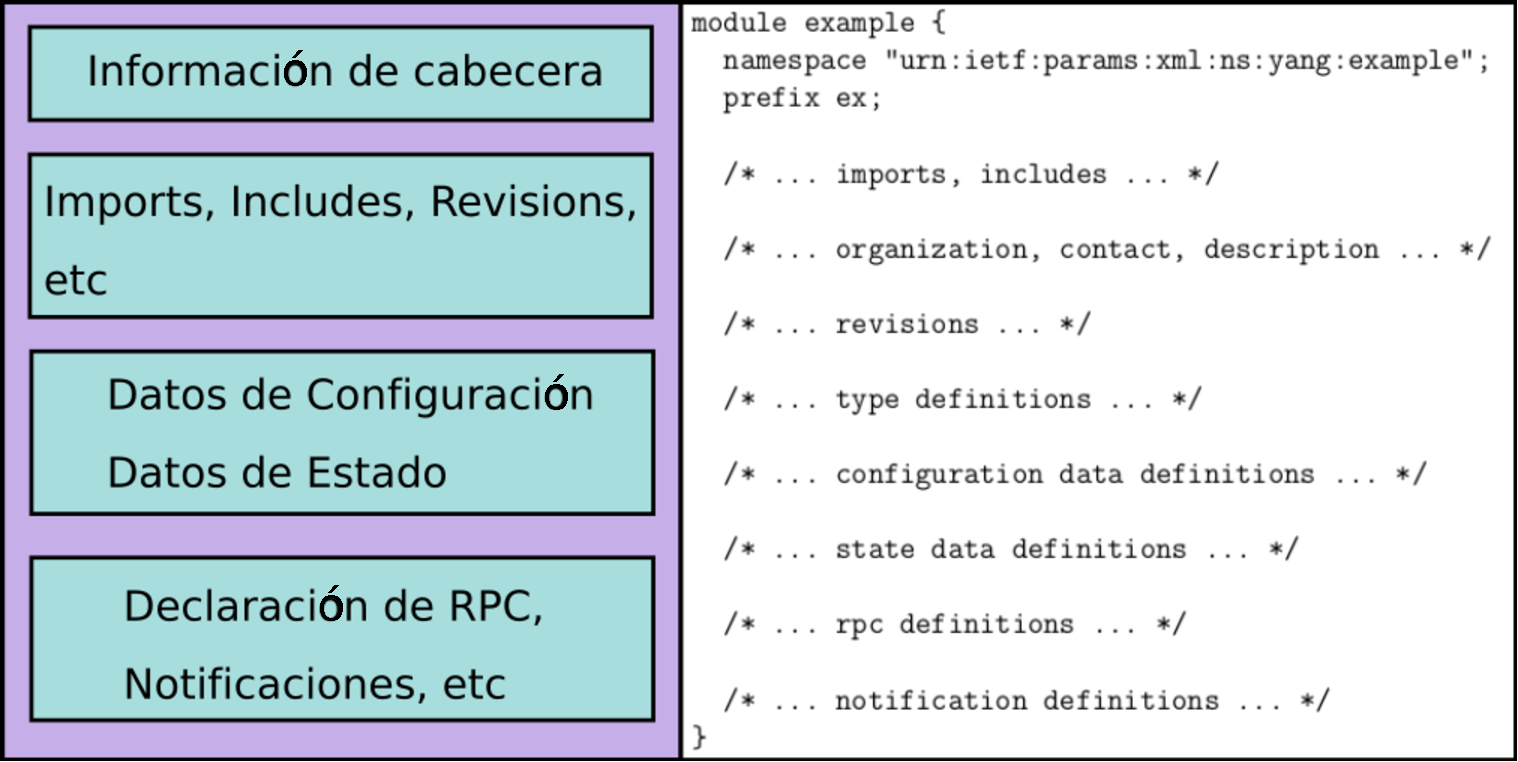
\includegraphics[scale=0.6]{Figures/estructura_modulo.pdf}
	\caption{Estructura de un módulo \textit{YANG}.}
	\label{fig:estructura_modulo}
  \end{figure}

  \subsubsection{Declaraciones y Definiciones de Datos}
  A continuación, se describen algunas sentencias que podría contener un módulo \textit{YANG}. Cada sentencia contiene la definición del tipo de dato y puede contener además algún valor para ese tipo de dato. Siempre representan a datos de configuración o datos de estado, realizando dicha distinción con la sentencia llamada \textit{“config“}.  

  \begin{itemize}
	\item \textbf{\textit{leaf}:} contiene un dato simple como un entero o un \textit{string}. Admite exactamente un valor para un tipo de dato particular y opcionalmente puede incluir una descripción. 
	\item \textbf{\textit{leaf-list}:} describe una secuencia de datos tipo \textit{leaf}. Cada \textit{leaf} admitirá un solo valor para el tipo de dato que especifique el \textit{leaf-list}.
	\item \textbf{\textit{container}:} es utilizado para agrupar datos lógicamente relacionados. Un \textit{container} no admite un valor, pero sí admite cualquier número de tipos de datos como \textit{leaf}, \textit{leaf-list}, \textit{container} o \textit{list}.
	\item \textbf{\textit{list}:} define una secuencia de tipo de datos donde cada tipo de dato es única, identificado por la sentencia \textit{key}. Puede contener múltiples identificadores \textit{key} y cualquier cantidad de tipo de datos \textit{leaf}, \textit{leaf-list}, \textit{container}, etc.
	\item \textbf{\textit{choices - cases}:} no describen algún tipo de dato, más bien ofrecen ramificaciones condicionales en la estructura del módulo. La sentencia \textit{choice} es una condición que asegura que, como máximo, se cumplira una de las declaraciones dadas por case.
\end{itemize}

Las declaraciones y sentencias descritas anteriormente pueden ser utilizadas en conjunto para poder formar una estructura de datos tipo árbol más compleja.
Además, \textit{YANG} admite la reutilización de sentencias mediante las declaraciones \textit{include} e \textit{import} reduciendo así los posibles errores en el modelado de datos.

\subsubsection{Identificador de instancia }
Cada dato en \textit{YANG}, así como el propio módulo, tiene un identificador único de instancia que se puede utilizar para referirse a él. Los identificadores se denominan \textit{namespace}, y admiten un prefijo para poder acortar el nombre. 
\\

Por ejemplo, Bjorklund \parencite{yangsystem}, definió un módulo \textit{YANG} para la administración de interfaces. Dicho modelo tiene una estructura de datos de tres niveles para una interfaz básica. En el nivel superior del modelo se encuentra definido el \textit{container} llamado \textit{“interface”}, seguido de la \textit{list “interface”} que contiene múltiples instancias de una interfaz, identificada por la \textit{key “name”}. Además, cada interfaz tiene una \textit{leaf “enabled”} que describe el estado de la misma. Un ejemplo de identificador para una instancia de \textit{“interface”} llamada \textit{“eth0”} puede verse en la figura \ref{fig:interfaceyang}.

\begin{figure}[htbp]
	\centering
	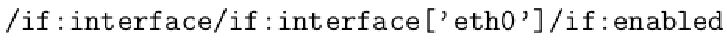
\includegraphics[scale=0.9]{Figures/interface-yang.pdf}
	\caption{Ejemplo de identificador de instancia en \textit{YANG}.}
	\label{fig:interfaceyang}
  \end{figure}

  \subsubsection{Funcionalidades}
  \textit{YANG} ofrece características especiales que lo distinguen de un documento \textit{JSON}, permitiéndole describir de forma eficiente las funcionalidades de la red. Estas características incluyen la validación de modelos, una forma estandarizada de extender a los módulos y compatibilidad entre las diferentes revisiones de los mismos. En esta sección, se analizaron las principales funcionalidades ofrecidas por \textit{YANG}.

  \begin{itemize}
	\item \textbf{Validación:} una de las características más importantes de \textit{YANG} es la posibilidad de validar automáticamente todos los datos descritos en el modelo. Resulta importante ya que la validación de los datos es una tarea difícil. Dicha afirmación está respaldada por el hecho de que introducir datos erróneos y tomarlos como válidos, está catalogada como la principal amenaza de seguridad según \textit{OWASP} \parencite{owasp}, organización sin ánimo de lucro a nivel mundial dedicada a mejorar la seguridad de las aplicaciones y del software en general. Cada dato introducido en el modelo \textit{YANG} puede ser validado semánticamente y sintácticamente. La validación de sintaxis es automática y garantiza que el dato contenga una secuencia de bytes válido, puesto que cada dato en el modelo tiene asociado un \textit{type} (string, int, uint, etc). Por otra parte, la validación semántica resulta más compleja y puede ser usada para describir dependencias entre datos. \textit{YANG} también admite sentencias como \textit{“when”} o \textit{“must”} que pueden ser usadas para evaluar condicionalmente un dato.  
	\item \textbf{Compatibilidad:} cada módulo admite la indicación de una revisión, esto permite a \textit{YANG} distinguir las versiones soportadas y adaptarse a la situación cuando la misma no es soportada. También, se describen reglas de actualización en los módulos que deben respetarse para mantener compatibilidad entre los modelos de datos anteriores. Por ejemplo, cualquier cambio en un módulo debe indicar una revisión en la cabecera, tanto el nombre del mismo como el namespace debe mantenerse, como así también las definiciones de datos obsoletas, lo que permite compatibilidad con modelos de datos anteriores. Esta característica permite a los módulos evolucionar con el paso del tiempo, sin romper aplicaciones existentes con versiones anteriores.
	\item \textbf{Extensión:} permite extender las funcionalidades de los módulos con nuevas definiciones de datos. Existen muchas razones por las cuales utilizar la extensión en \textit{YANG}, como por ejemplo, desarrollar un nuevo módulo a partir de uno existente o con el fin de reducir errores reutilizando un módulo funcional. Una ventaja importante que tiene utilizar la extensión, es que al agregar nueva información en un módulo, se mantiene compatibilidad con el heredado.
\end{itemize}

\subsection{Redes Ópticas de Transporte}
La explosión del tráfico digital provocado por los nuevos enfoques como \textit{Big Data} o el \textit{Streaming}, y los requerimientos de los usuarios donde existe un constante crecimiento de aplicaciones con alta demanda de ancho de banda, requieren de una nueva tecnología de transporte que pueda ocuparse de los patrones de tráfico y los contenidos de datos modernos. Para ello, se han realizados numerosos avances en los últimos años referente al plano de control y el plano de datos de las redes ópticas \parencite{redesopticas}, surgiendo protocolos como SONET o OTN. En esta sección, se analiza las redes ópticas, utilizadas para el transporte de los datos como así también los dispositivos que funcionan sobre dichas redes. 
\\

Una red de transporte óptica, es un tipo de red de comunicaciones de datos que utiliza la luz como medio de transporte para la información \parencite{redesopticasdef}. A diferencia de las redes basadas en cobre, los pulsos de luz de una red óptica pueden transportarse a una distancia considerable e incluso regenerarse a través de un dispositivo repetidor óptico. Después de que una señal óptica es recibida en su red de destino, la misma se convierte en una señal eléctrica a través de un receptor óptico, para luego ser enviado al nodo de la capa de paquetes. 
\\

Un sistema de comunicaciones ópticas puede incluir diversos dispositivos, como ser:

\begin{itemize}
	\item \textbf{Amplificadores ópticos} 
	\item \textbf{\textit{Switches} ópticos,} encargados de conmutar de un canal a otro.
	\item \textbf{Divisores de luz,} cuya tarea comprende dividir la señal en diferentes caminos de fibra óptica.
	\item \textbf{Fibra óptica,} que cumple de medio de transporte de la información entre los diferentes equipos.
	\item \textbf{\textit{Transponders} y \textit{Muxponders},} encargados de enviar y recibir las señales ópticas por las fibras. Generalmente son caracterizados por el ancho de banda que pueden transportar y la distancia que puede alcanzar la transmisión.
\end{itemize}

\subsubsection{\textit{Transponders} y \textit{Muxponders}}
El \textit{transponder}, es un dispositivo que recibe múltiples señales ópticas a través de sus puertos clientes, dichas señales ópticas pueden tratarse de servicios diferentes como por ejemplo, \textit{Ethernet}, \textit{SONET}, \textit{OTN}, entre otros. Luego, transforma estas señales en flujos de datos eléctricos, las procesa y regenera las mismas para nuevamente convertirlas en señales ópticas compatibles con el estándar \textit{ITU}. De esta forma, realiza la función de recepción, amplificación y reemisión de una señal óptica en un proceso que comúnmente se denomina \textit{optical electrical optical} (OEO) \parencite{transpondermux}.
\\

La figura \ref{fig:transponder} ejemplifica el proceso \textit{OEO} típico de un \textit{transponder}.

\begin{figure}[H]
	\centering
	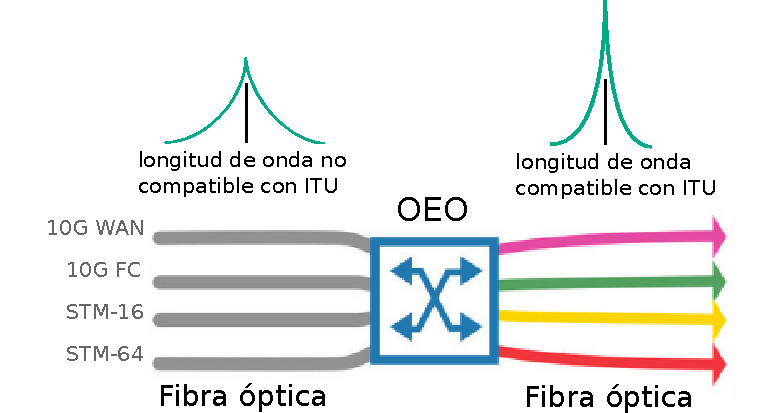
\includegraphics[scale=0.9]{Figures/transponder.pdf}
	\caption{Funcionamiento básico de un \textit{transponder}.}
	\label{fig:transponder}
  \end{figure}

  Por otra parte, los \textit{muxponders} realizan una función similar a los \textit{transponders}. También incluyen el proceso \textit{OEO}, con la diferencia de que combinan múltiples servicios en una sola longitud de onda que luego se multiplexan en la misma fibra \parencite{transpondermux}. Por lo tanto, en lugar de asignar a cada servicio una longitud de onda dedicada, permite que varios servicios diferentes compartan la misma longitud de onda. Estos dispositivos maximizan la utilización de la fibra y ofrecen soluciones de bajo costo para empresas y transportistas. La figura \ref{fig:muxponder} muestra el comportamiento de un \textit{muxponder}.

  \begin{figure}[htbp]
	\centering
	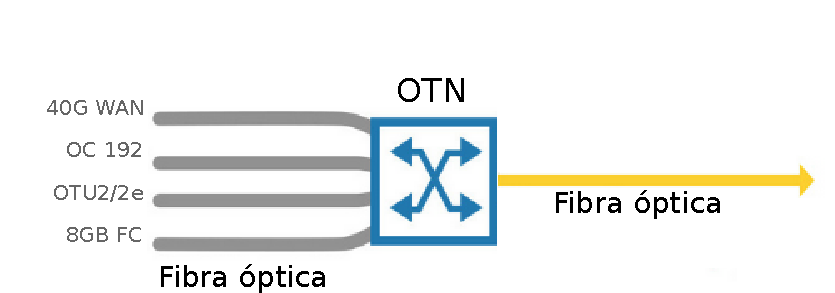
\includegraphics[scale=0.9]{Figures/muxponder.pdf}
	\caption{Funcionamiento básico de un \textit{muxponder}.}
	\label{fig:muxponder}
  \end{figure}

  \subsubsection{Aplicaciones}
  Resulta importante ahora separar la red en dos capas diferentes: la capa de paquetes o de \textit{IP/MPLS}, y la capa óptica o de transporte \parencite{capasredess}. La figura \ref{fig:capasredes} muestra dicha separación.  Los dispositivos mencionados anteriormente se utilizan en la capa de transporte mientras que los \textit{routers} y \textit{switches} convencionales se encuentran en la capa \textit{IP/MPLS}.
  \\

La función que tienen los \textit{muxponders} es la de proveer una conexión lógica entre los diferentes \textit{routers}, quienes podrían estar separados por enormes distancias donde los protocolos como \textit{Ethernet} no proveen un buen servicio de transporte. 
\\

De esta forma, los dispositivos de la capa \textit{IP/MPLS} tienen conocimiento de sus vecinos pero no de la forma en la que se encuentran conectados ni de cómo se está realizando dicha comunicación, mientras que los equipos de la capa óptica esencialmente emparejan a los dispositivos de la capa \textit{IP/MPLS}, pero sin tener conocimiento sobre los diferentes servicios que se prestan. 

\begin{figure}[htbp]
	\centering
	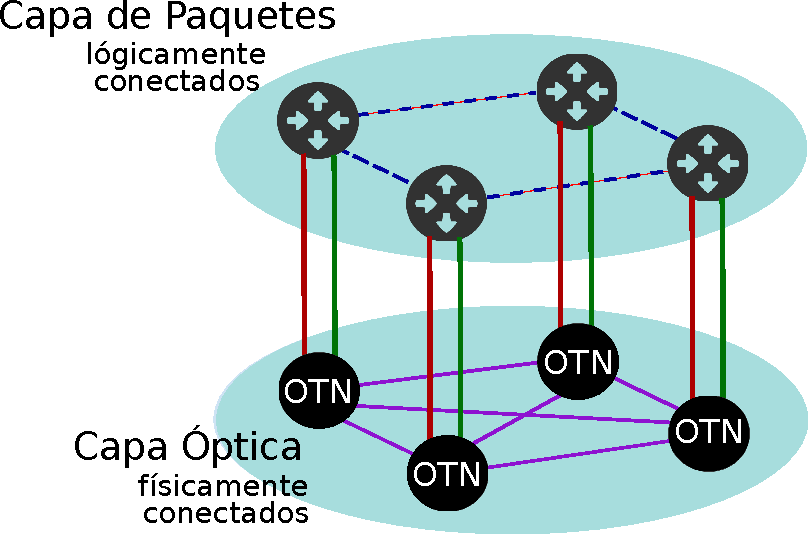
\includegraphics[scale=0.8]{Figures/capasredes.pdf}
	\caption{Separación de la red en capa de paquetes y capa de transporte.}
	\label{fig:capasredes}
  \end{figure}